\documentclass[11pt]{article}

\usepackage{graphicx}
\usepackage{float}
\usepackage{amsmath}

\DeclareMathOperator*{\argmin}{arg\,min}
\DeclareMathOperator*{\argmax}{arg\,max}


\begin{document}

\section{Intro}
	\textbf{Manifold Mesh}: Made of manifold triangles
\begin{itemize}
	\item edges have at most two incident triangles	
	\item edges with only one incident triangle form a mesh boundary	
	\item faces incident to an edge form open/closed fan
\end{itemize}


\paragraph{Point Cloud} Collection of points in the 3D space
\begin{itemize}
	\item point cloud are interpreted as point-wise sampling of an underlying unknown surface
	\item Oriented point cloud has a norm for each point
\end{itemize}
Often come from depth sensors, can be very noisy.


\section{Metric Geometry}
Given a sphere, how do we compute distance from \textit{x} to \textit{y}?
\begin{itemize}
	\item \textbf{Euclidean Distance:} straight walk from x to y
	\item \textbf{Geodesic Distance:} walk on the surface, from x to y
\end{itemize}

\subsection{Distances}
\begin{itemize}
	\item Distances in $R^2$
		\paragraph{Euclidean Distance}
		\begin{equation}
			||a-b||_2 = ((a_x - b_x)^2 + (a_y - b_y)^{2})^\frac{1}{2}
		\end{equation}

		\paragraph{$L_p$ Distance}
		\begin{equation}
			||a-b||_p = ((a_x - b_x)^p + (a_y - b_y)^{p})^\frac{1}{p}
		\end{equation}

\item $L_p$ distance between vectors in $R^k$
		\begin{equation}
			||a-b||_p = (\sum_{i=1}^K (a_i - b_i)^p)^{\frac{1}{p}})
			\end{equation}



\begin{figure}[H]
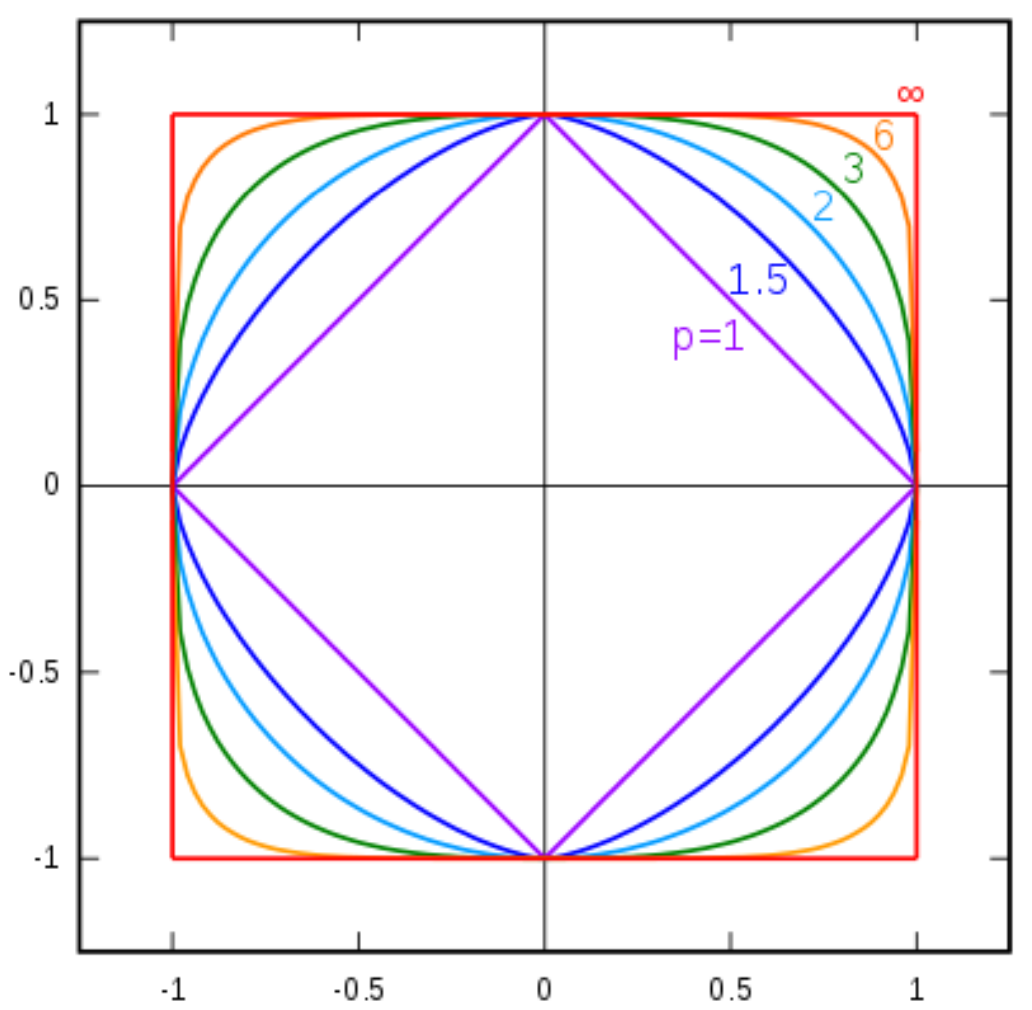
\includegraphics[scale=0.3]{res/images/lp.png}
\centering
\caption{$L_p$ unit balls}
\label{}
\end{figure}
\end{itemize}

\subsection{Metric Spaces}
A \textit{metric space} is a pair \textit{(object, distance)}.\\
A set $M$ is a metric space if for every pair of points $x,y \in M$ there is a \textit{metric} (distance) function $d_M: M \times M: R_+$ such that:
\begin{itemize}
	\item $d_M(x,y)=0 \Leftrightarrow x=y$ (identity of indiscernibles)
	\item $d_M(x,y)=d_M(y,x)$ (symmetry)
	\item $d_M(x,y) \leq d_M(x,z) + d_M(z,y)$ for any $x,y,z \in M$ (triangle inequality)
\end{itemize}
In this course, a metric space is defined as the pair $(M,d_M)$
E.g:
\begin{itemize}
	\item Sphere with Euclidean distance is $(S^2, d_{L_2})$
	\item Sphere with Geodesic distance is $(S^2, d_g)$
\end{itemize}
Examples of metric spaces:
\begin{itemize}
	\item $X=R, d_X(x,y) = |x-y|$
	\item $X=A \subset R^k, d_X(x,y) = ||x-y||_2$
	\item $X=R, d_X(x,y) = log(|x-y|+1)$
	\item $X = A \times B, d_X((a1,b1),(a2,b2)) = \sqrt{d_A(a1,a2)^2 + d_B(b1,b2)^2}$
	\item $X=$any set, $d_X(x,y) = \begin{cases}
		0 & \mbox{if } x=y\\
		1 & \mbox{if } x \neq y\\
	\end{cases}$
\end{itemize}

\subsection{Geodesic Isolines}
Identify a set of points $x \in X$ at the same distance (according to $d_g$) to some reference point $y \in X$.


\subsection{Farthest Point Sampling}
\begin{itemize}
	\item fix $n$ and $S^{(0)} = y$ for some $y \in X$.
	\item repeat until $k = n$:
	\begin{itemize}
		\item At step $k$, given $S^{(k-1)}$, select $x \in X$ such that\\
			$x = \argmax_{x \in X} d_X(x,S^{(k-1)})$
		\item $S^(k) = S^{(k-1)} \cup x	$
	\end{itemize}
\end{itemize}

\subsection{Voronoi Decomposition}
For a given sampling S, associated \textit{Voronoi regions} are defined as:
\begin{equation}
	V_i(S) = \{x \in X : d_X(x, x_i) < d_X(x, x_j), x_{j \neq i} \in S\}
\end{equation}

Voronoi regions can be implemented either for meshes and point clouds, using the Euclidean distance and using a farthest point sampling $S$.

\subsection{Ambient Space and Restriciton}
If $A$ is a metric space and $X \subset A$ then $A$ cis called \textit{ambient space} for $X$.\\
A metric on $X$ can be obtained by the \textit{restriction} $d_X = d_{A|X}$ such that:
\begin{equation}
	d_X(x,y) = d_A(x,y)
\end{equation}
for all $x,y \in X$

\subsection{Isometries}
Given two metric spaces ($M,d_M$) and ($N,d_N$), a bijective map $f:M \rightarrow N$ is an \textbf{isometry} iff:
\begin{equation}
	d_M(x,y) = d_N(f(x),f(y))
\end{equation}
for any $x,y \in M$

if $d_M = ||\cdot||_2$ and $d_N = ||\cdot||_2$ it is a \textit{rigid isometry}, meaning that we preserve the Euclidean distances, hence we're only rotating or translating the shape.

\textbf{Quasi Isometries}: non rigid isometries, where 
\begin{equation}
	d_M(x,y) \approx d_N(f(x), f(y))
\end{equation}
($d_M$ and $d_N$ are geodesic distance functions)

\begin{figure}[H]
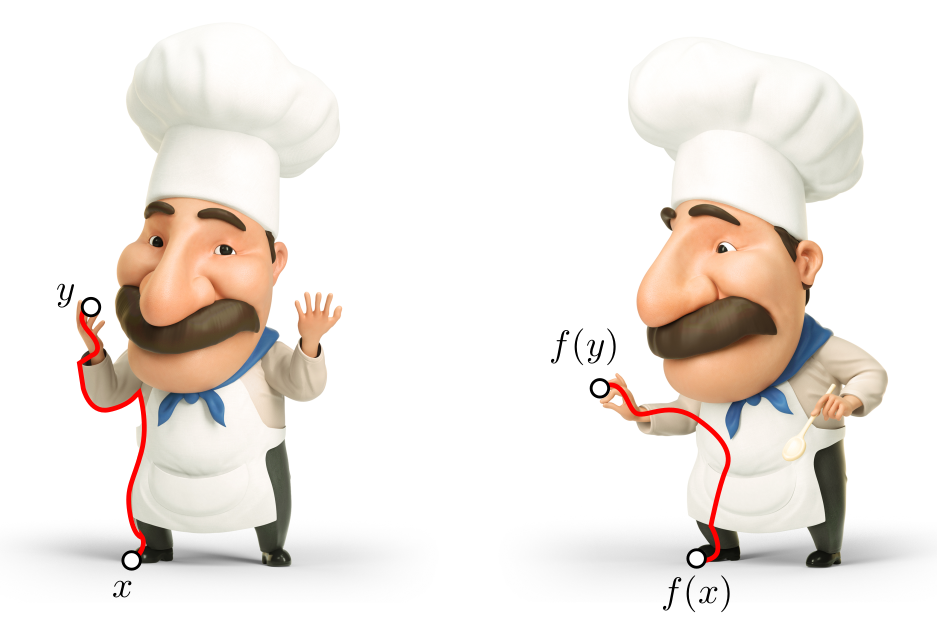
\includegraphics[scale=0.3]{res/images/quasi_iso.png}
\centering
\caption{non-rigid isometry}
\label{}
\end{figure}

Isometry can be seen as an \textbf{equivalence} relation, since it is:
\begin{itemize}
	\item \textbf{reflective:} $a=a$
	\item \textbf{symmetric:} $a=b \Rightarrow b=a$
	\item \textbf{transitive:} $a=b  \wedge b=c \Rightarrow a=c$
\end{itemize}
meaning that we can think of \textbf{isometric shapes} as being the \textbf{same shape}.

\subsection{Distance}
There are many notions of \textbf{distance between shapes}.
\textbf{Distance from point $x$ to set $A \subseteq (X, d_X)$:}
\begin{equation}
	dist_X(x,A) = \min_{y \in A} d_X(x,y)
\end{equation}

\begin{figure}[H]
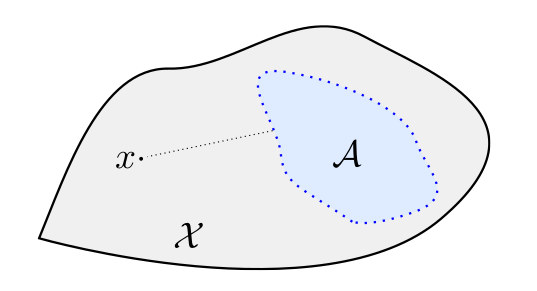
\includegraphics[scale=0.3]{res/images/dist.png}
\centering
\label{}
\end{figure}

\subsection{Hausdorff Distance}
The \textbf{Hausdorff Distance} is defined between \textit{subsets of a metric space}
Given two subsets $X,Y \subset (Z,d_Z)$
\begin{equation}
	d_{H}^{Z} = \max \{\max_{x \in X} dist_Z(x,Y), \max_{y \in Y} dist_Z(y,X)\}
\end{equation}

\begin{figure}[H]
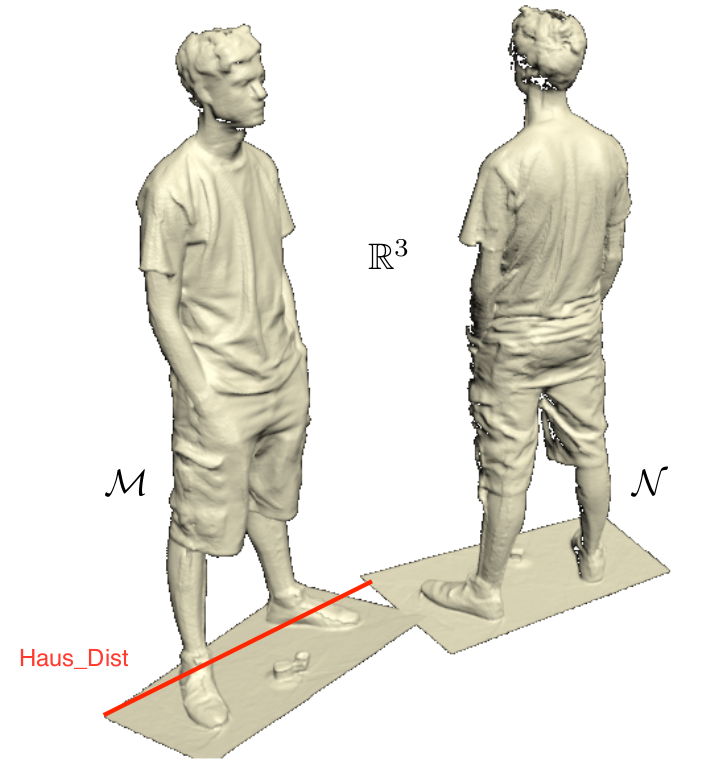
\includegraphics[scale=0.3]{res/images/haus_dist.png}
\centering
\caption{Hausdorff distance, rigid case}
\label{}
\end{figure}	
To minimize the Hausdorff distance between these two shapes, we can overlap them.
It is useful indeed to \textit{compare rigid shapes}.


























\end{document}